\begin{frame}{Introduction}
    \begin{itemize}
        \item A user interface (UI) to match images of the same location from distinct datasets
    \end{itemize}
\end{frame}

\begin{frame}{Introduction}
    \begin{itemize}
        \item A user interface (UI) to match images of the same location from distinct datasets
        \item An Application Programming Interface (API) to process data created by the UI
    \end{itemize}
\end{frame}

\begin{frame}{Introduction}
    \begin{figure}[H]
      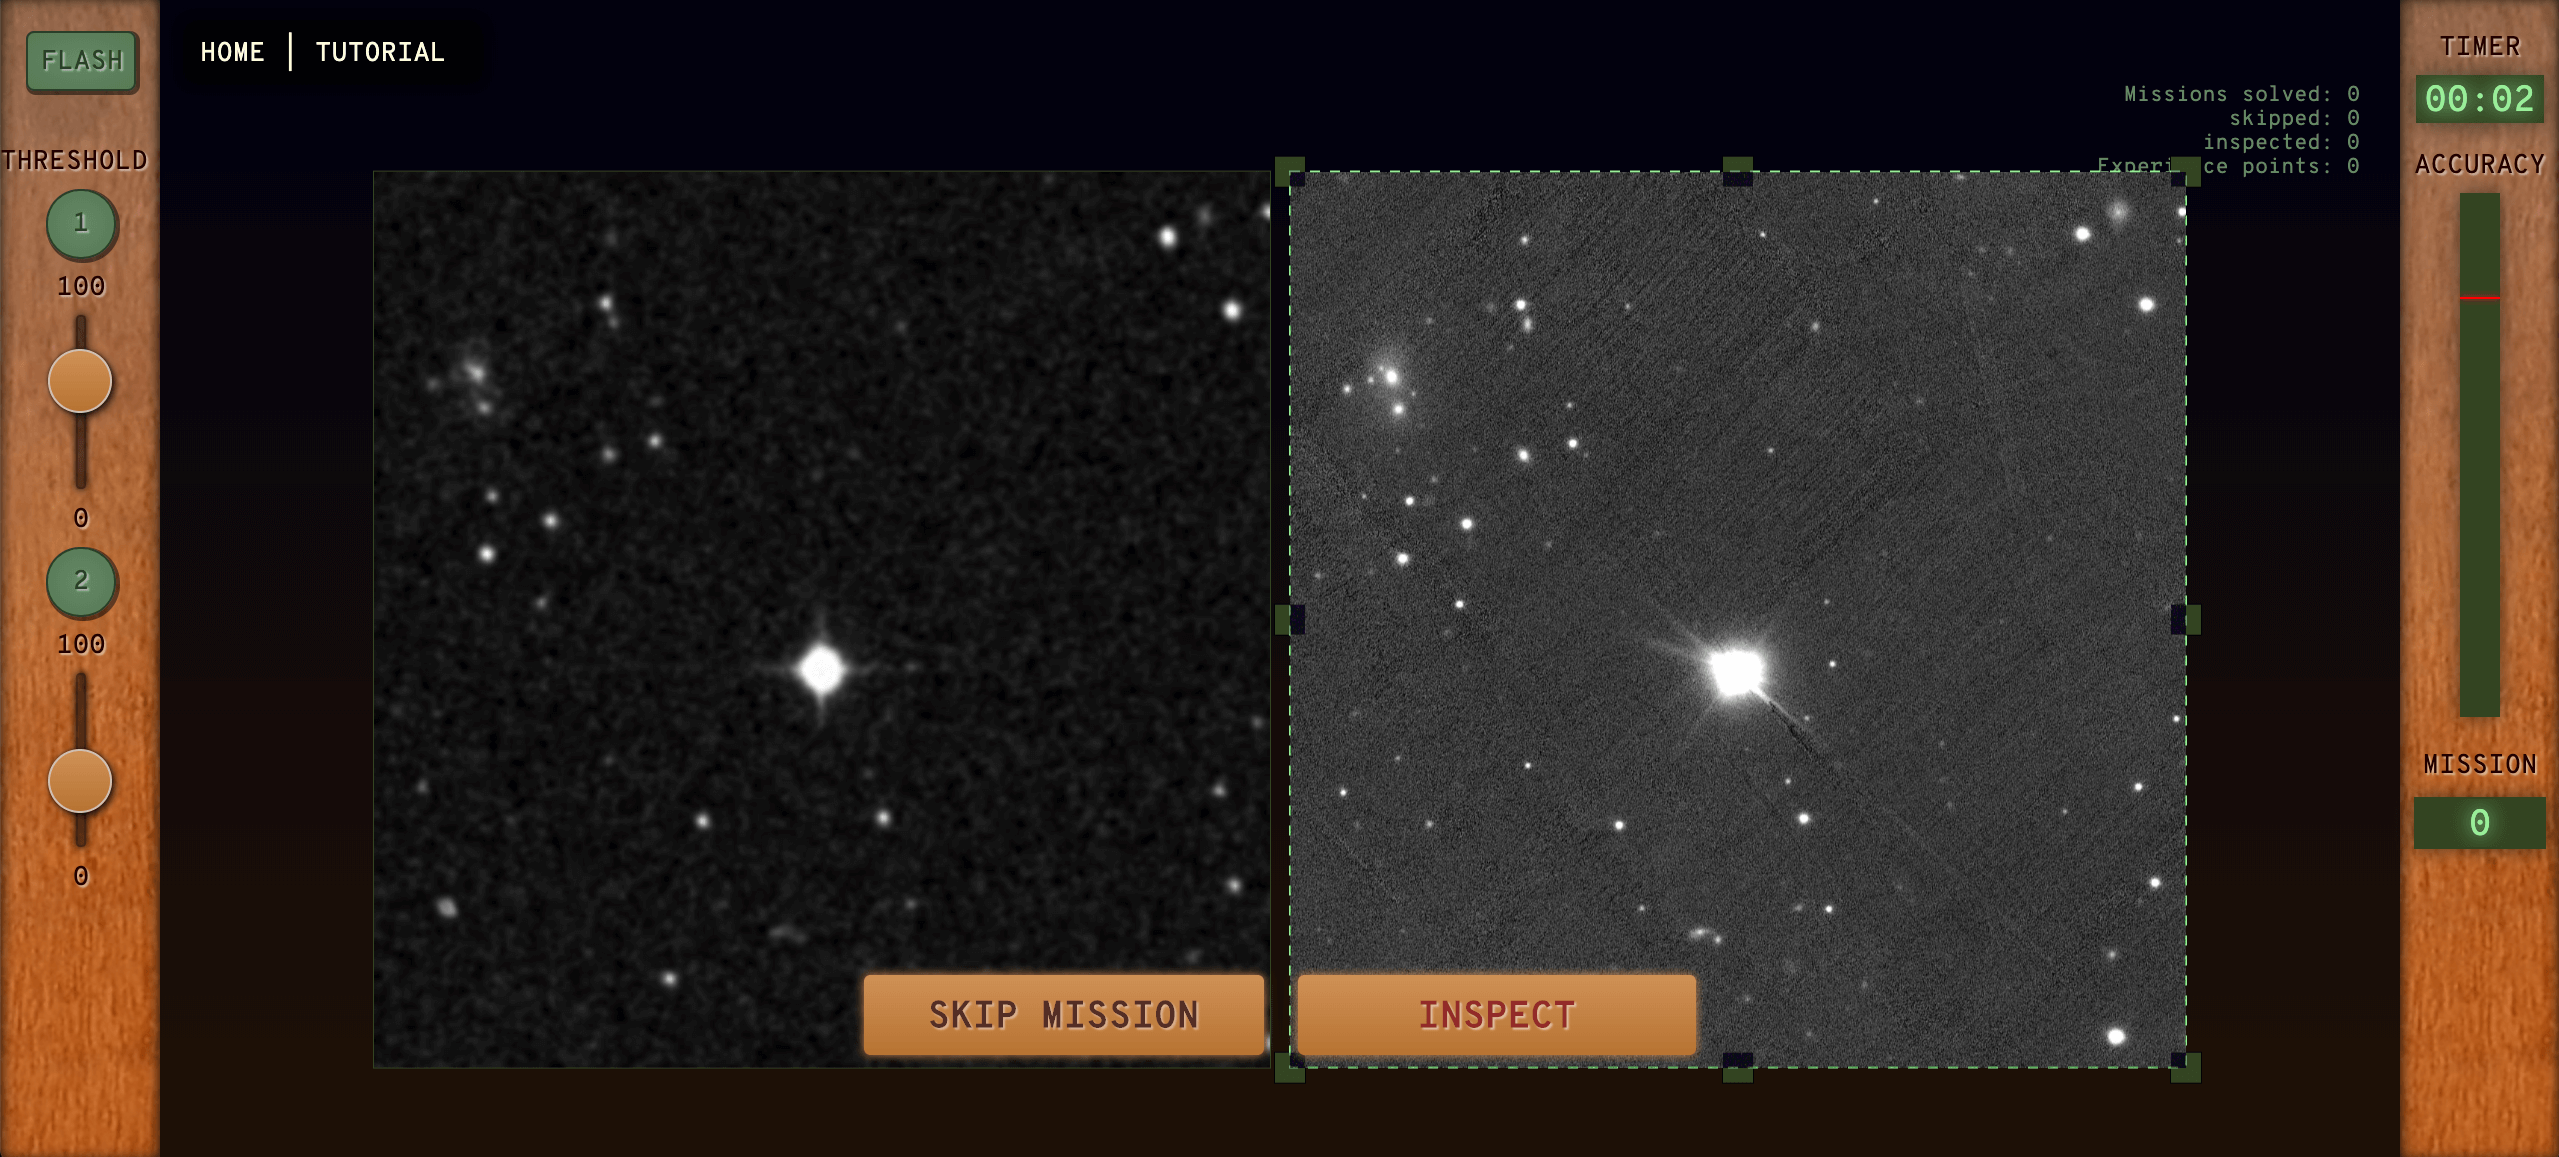
\includegraphics[
            width=\textwidth,
            keepaspectratio
      ]{report/images/ml-blink-ui-main-screen.png}
      \caption{UI used to conduct the case study.}
    \end{figure}
\end{frame}

\begin{frame}{Matching Accuracy}
    \begin{itemize}
        \item Accuracy threshold to determine whether a mission has an anomaly(s)
    \end{itemize}
\end{frame}

\begin{frame}{Matching Accuracy}
    \begin{itemize}
        \item Accuracy threshold to determine whether a mission has an anomaly(s)
        \item Accuracy threshold fixed at 80\%
    \end{itemize}
\end{frame}

\begin{frame}{Matching Accuracy}
    \begin{itemize}
        \item Accuracy threshold to determine whether a mission has an anomaly(s)
        \item Accuracy threshold fixed at 80\%
        \item Artificial anomalies were created
    \end{itemize}
\end{frame}

\begin{frame}{Matching Accuracy}
    \begin{figure}[H]
        \begin{subfigure}{.5\textwidth}
          \centering
          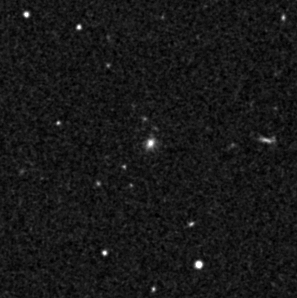
\includegraphics[
                width=\textwidth,
                height=0.40\textheight,
                keepaspectratio
            ]{report/images/fake-anomalies/usno-13-blue1.png}
          \caption{\usno}
        \end{subfigure}%
        \begin{subfigure}{.5\textwidth}
          \centering
          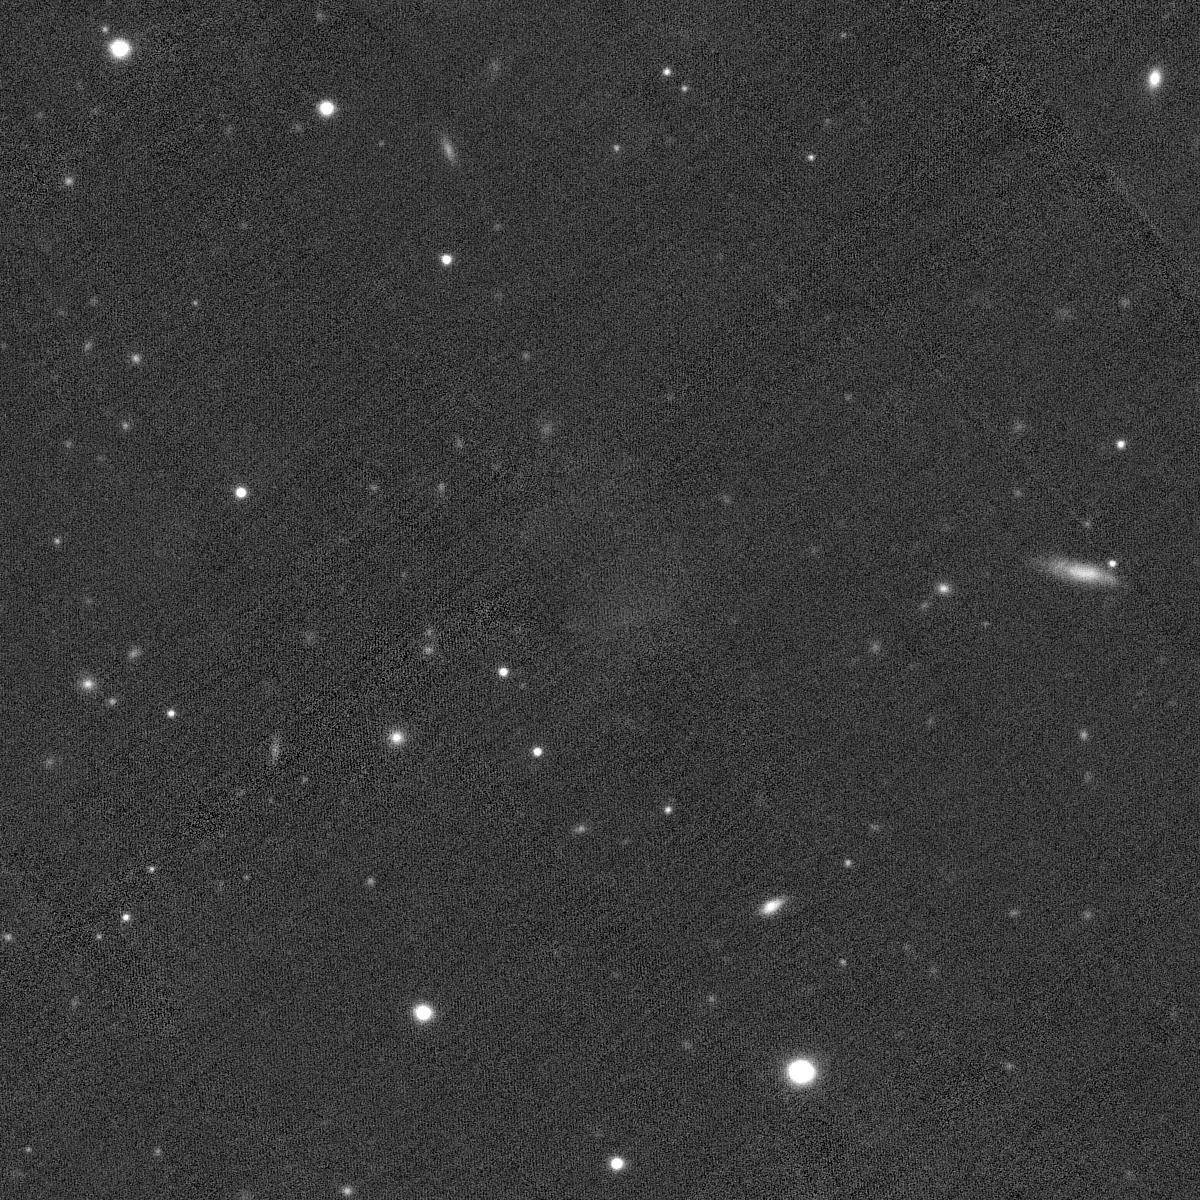
\includegraphics[
                width=\textwidth,
                height=0.40\textheight,
                keepaspectratio
          ]{report/images/fake-anomalies/panstarr-13-g.png}
          \caption{\panstarrs}
        \end{subfigure}
        \caption{Images manually altered taken from the same location in the night sky from \usno and \panstarrs respectively. An object close to the center of the \panstarrs image has been replaced by the image's background, while the \usno image is unaltered.}
    \end{figure}
\end{frame}